% !TeX program = pdflatex
\documentclass[11pt,twoside]{article}

% =============================================================================
% PACKAGES
% =============================================================================
\usepackage[utf8]{inputenc}
\usepackage[T1]{fontenc}
\usepackage[margin=1in,inner=1.1in,outer=0.9in,headheight=14pt]{geometry}
\usepackage{enumitem}
\usepackage{booktabs}
\usepackage{longtable}
\usepackage{tabularx}
\usepackage{multirow}
\usepackage{xcolor}
\usepackage{array}
\usepackage{amssymb}
\usepackage{tikz}
\usepackage{pgfplots}
\usepackage{graphicx}
\usepackage{fancyhdr}
\usepackage{titlesec}
\usepackage{tcolorbox}
\usepackage{calc}
\usepackage{float}
\usepackage{wrapfig}
\usepackage{colortbl}
\usepackage{siunitx}
\usepackage{pifont}
\usepackage{multicol}
\usepackage{caption}
\usepackage[hidelinks,colorlinks=true,linkcolor=darkgreen!70!black,urlcolor=blue!70!black]{hyperref}

% =============================================================================
% TIKZ LIBRARIES
% =============================================================================
\usetikzlibrary{shapes.geometric, arrows.meta, positioning, calc, patterns, decorations.pathmorphing, shadows, backgrounds}
\pgfplotsset{compat=1.18}

% =============================================================================
% COLOR DEFINITIONS
% =============================================================================
\definecolor{watermelongreen}{RGB}{34, 139, 34}
\definecolor{watermelonpink}{RGB}{255, 105, 180}
\definecolor{watermelonrind}{RGB}{144, 238, 144}
\definecolor{soilbrown}{RGB}{139, 90, 43}
\definecolor{sunlightyellow}{RGB}{255, 215, 0}
\definecolor{alertred}{RGB}{220, 53, 69}
\definecolor{warningorange}{RGB}{255, 153, 0}
\definecolor{successgreen}{RGB}{40, 167, 69}
\definecolor{infoblue}{RGB}{23, 162, 184}
\definecolor{lightgray}{RGB}{248, 249, 250}
\definecolor{darkgreen}{RGB}{0, 100, 0}

% =============================================================================
% TCOLORBOX STYLES
% =============================================================================
\tcbuselibrary{skins,breakable}

\newtcolorbox{criticalbox}{
  colback=alertred!10,
  colframe=alertred,
  fonttitle=\bfseries,
  title={\ding{54} Critical},
  breakable,
  enhanced,
  boxrule=1pt,
  left=5pt,
  right=5pt,
  top=5pt,
  bottom=5pt
}

\newtcolorbox{warningbox}{
  colback=warningorange!10,
  colframe=warningorange,
  fonttitle=\bfseries,
  title={\ding{43} Warning},
  breakable,
  enhanced,
  boxrule=1pt,
  left=5pt,
  right=5pt,
  top=5pt,
  bottom=5pt
}

\newtcolorbox{tipbox}{
  colback=successgreen!10,
  colframe=successgreen,
  fonttitle=\bfseries,
  title={\ding{52} Pro Tip},
  breakable,
  enhanced,
  boxrule=1pt,
  left=5pt,
  right=5pt,
  top=5pt,
  bottom=5pt
}

\newtcolorbox{infobox}{
  colback=infoblue!10,
  colframe=infoblue,
  fonttitle=\bfseries,
  title={\ding{46} Information},
  breakable,
  enhanced,
  boxrule=1pt,
  left=5pt,
  right=5pt,
  top=5pt,
  bottom=5pt
}

\newtcolorbox{procedurebox}[1][]{
  colback=lightgray,
  colframe=darkgreen,
  fonttitle=\bfseries,
  title={#1},
  breakable,
  enhanced,
  boxrule=1pt,
  left=5pt,
  right=5pt,
  top=5pt,
  bottom=5pt
}

% =============================================================================
% LIST FORMATTING
% =============================================================================
\setlist[itemize]{leftmargin=*, itemsep=0.35em, topsep=0.35em}
\setlist[enumerate]{leftmargin=*, itemsep=0.35em, topsep=0.35em}
\setlist[itemize,2]{label=\textendash}
\setlist[itemize,3]{label=\textasteriskcentered}

% =============================================================================
% SECTION FORMATTING
% =============================================================================
\titleformat{\section}
  {\normalfont\Large\bfseries\color{watermelongreen}}
  {\thesection}{1em}{}[\titlerule]
  
\titleformat{\subsection}
  {\normalfont\large\bfseries\color{darkgreen}}
  {\thesubsection}{1em}{}

\titleformat{\subsubsection}
  {\normalfont\normalsize\bfseries\color{darkgreen!80}}
  {\thesubsubsection}{1em}{}

% =============================================================================
% HEADER AND FOOTER
% =============================================================================
\pagestyle{fancy}
\fancyhf{}
\fancyhead[LE,RO]{\thepage}
\fancyhead[RE]{\textit{Bradford Watermelon Balcony Run Book}}
\fancyhead[LO]{\textit{\leftmark}}
\renewcommand{\headrulewidth}{0.4pt}
\renewcommand{\footrulewidth}{0pt}

% =============================================================================
% CUSTOM COMMANDS
% =============================================================================
\newcommand{\cb}{\(\square\)\hspace{0.5em}}
\newcommand{\cbcheck}{\ding{51}\hspace{0.5em}}
\newcommand{\degree}{$^\circ$}
\newcommand{\tempf}[1]{#1\,\degree F}
\newcommand{\gallon}[1]{#1\,gal}
\newcommand{\inch}[1]{#1\,in}
\newcommand{\ft}[1]{#1\,ft}

% =============================================================================
% DOCUMENT INFORMATION
% =============================================================================
\title{%
  \vspace{-1cm}
  \begin{tikzpicture}[remember picture, overlay]
    \fill[watermelongreen!20] (-8,-2) rectangle (8,3);
    \foreach \i in {1,...,15} {
      \fill[watermelongreen!\the\numexpr40+\i*3\relax, opacity=0.3] 
        ({-6+rand*12}, {-1+rand*3}) circle ({0.1+rand*0.3});
    }
  \end{tikzpicture}
  {\Huge\bfseries\color{watermelongreen} Bradford Watermelon}\\[0.3cm]
  {\Huge\bfseries\color{darkgreen} Balcony Run Book}\\[0.5cm]
  {\Large\color{soilbrown} Comprehensive Growing Guide for Container Cultivation}\\[0.3cm]
  {\large Lithia Springs, Georgia (Ground-Level Balcony)}\\[0.2cm]
  {\normalsize USDA Hardiness Zone 8a}
}
\author{%
  \textit{Version 2.0 --- Enhanced Edition}
}
\date{\today}

% =============================================================================
% BEGIN DOCUMENT
% =============================================================================
\begin{document}
\maketitle
\thispagestyle{empty}

% =============================================================================
% ABSTRACT
% =============================================================================
\begin{abstract}
\noindent This comprehensive run book provides an end-to-end, execution-oriented procedure for successfully growing Bradford (Bradford Family) heirloom watermelons in containers on a ground-level balcony in Lithia Springs, Georgia. The guide encompasses complete planning windows with detailed timelines, a procurement-ready materials and tools section with sourcing recommendations, phase-by-phase operating procedures from seed selection through harvest, integrated pest management protocols, comprehensive troubleshooting guidance, detailed nutrient management schedules, weather contingency plans, post-harvest handling procedures, and a rigorous pre-flight readiness review to minimize failure risk before transplanting. This enhanced edition includes visual diagrams, decision flowcharts, and expanded reference appendices for the most successful Bradford watermelon cultivation experience.
\end{abstract}

\vspace{1cm}

% =============================================================================
% DOCUMENT OVERVIEW DIAGRAM
% =============================================================================
\begin{center}
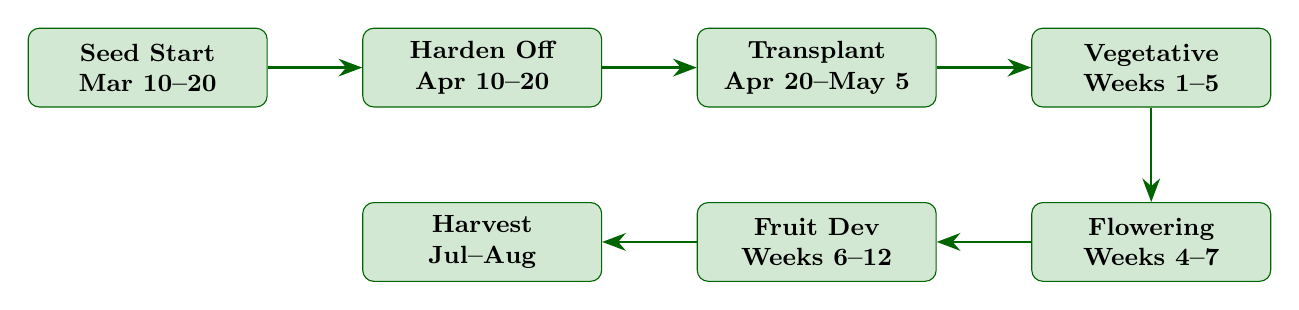
\begin{tikzpicture}[
  node distance=1.2cm,
  phase/.style={rectangle, rounded corners, draw=darkgreen, fill=watermelongreen!20, 
                text width=2.8cm, minimum height=1cm, align=center, font=\small\bfseries},
  arrow/.style={-{Stealth[length=3mm]}, thick, darkgreen}
]
  \node[phase] (seed) {Seed Start\\Mar 10--20};
  \node[phase, right=of seed] (harden) {Harden Off\\Apr 10--20};
  \node[phase, right=of harden] (transplant) {Transplant\\Apr 20--May 5};
  \node[phase, right=of transplant] (grow) {Vegetative\\Weeks 1--5};
  \node[phase, below=of grow] (flower) {Flowering\\Weeks 4--7};
  \node[phase, left=of flower] (fruit) {Fruit Dev\\Weeks 6--12};
  \node[phase, left=of fruit] (harvest) {Harvest\\Jul--Aug};
  
  \draw[arrow] (seed) -- (harden);
  \draw[arrow] (harden) -- (transplant);
  \draw[arrow] (transplant) -- (grow);
  \draw[arrow] (grow) -- (flower);
  \draw[arrow] (flower) -- (fruit);
  \draw[arrow] (fruit) -- (harvest);
\end{tikzpicture}
\end{center}

\newpage
\tableofcontents
\newpage

% =============================================================================
% SECTION 1: BRADFORD WATERMELON BACKGROUND
% =============================================================================
\section{Bradford Watermelon: Heritage and Characteristics}

\subsection{Historical Significance}

The Bradford watermelon represents one of America's most celebrated heirloom varieties, with a lineage tracing back to the antebellum South. Developed by the Bradford family in Sumter County, South Carolina, this variety gained legendary status for its exceptional sweetness and delicate texture throughout the 19th and early 20th centuries.

\begin{infobox}
The Bradford watermelon was so prized that it was considered too fragile for commercial transport, leading to its near-extinction by the mid-20th century. The variety was preserved by the Bradford family through generations and reintroduced to the public in 2013 by Nat Bradford, the eighth-generation descendant of the original breeder.
\end{infobox}

\subsection{Varietal Characteristics}

\begin{table}[H]
\centering
\caption{Bradford Watermelon Specifications}
\begin{tabular}{@{}p{4cm}p{9cm}@{}}
\toprule
\textbf{Characteristic} & \textbf{Description} \\
\midrule
Days to Maturity & 85--100 days from transplant \\
Fruit Size & 15--25 lbs typical; up to 40 lbs possible in ideal conditions \\
Shape & Oblong to oval \\
Rind & Light green with darker green stripes; thin and fragile \\
Flesh & Deep red, exceptionally sweet, fine-grained texture \\
Seeds & Dark brown to black; heirloom (open-pollinated) \\
Brix Level & 12--14\degree{} (higher than most commercial varieties) \\
Vine Type & Long, vigorous vines; 12--15 ft spread typical \\
Pollination & Monoecious; requires insect pollination or hand-pollination \\
\bottomrule
\end{tabular}
\end{table}

\subsection{Why Container Growing Requires Special Care}

Bradford watermelons evolved for open-field cultivation with unlimited root space. Container growing presents unique challenges that this run book addresses through specific adaptations.

\begin{itemize}
  \item \textbf{Root volume limitation:} Large containers and optimized media compensate for restricted root space
  \item \textbf{Nutrient depletion:} Structured feeding program replaces natural soil nutrient cycling
  \item \textbf{Temperature fluctuation:} Container walls heat faster than ground soil, requiring monitoring
  \item \textbf{Water stress:} Smaller soil volume demands consistent irrigation management
  \item \textbf{Fruit load management:} Strict thinning maintains quality despite reduced plant resources
\end{itemize}

% =============================================================================
% SECTION 2: OPERATING PARAMETERS
% =============================================================================
\section{Operating Parameters for Lithia Springs, GA}

\subsection{Climate Profile}

\begin{table}[H]
\centering
\caption{Lithia Springs Climate Data Relevant to Watermelon Cultivation}
\begin{tabular}{@{}p{5cm}p{8cm}@{}}
\toprule
\textbf{Parameter} & \textbf{Value/Range} \\
\midrule
USDA Hardiness Zone & 8a (10--15\degree F minimum) \\
Average Last Spring Frost & March 15--April 5 (verify annually) \\
Average First Fall Frost & November 5--15 \\
Frost-Free Growing Season & Approximately 210--230 days \\
Summer High Temperatures & 85--95\degree F typical; 100\degree F+ possible \\
Summer Humidity & 60--80\% relative humidity \\
Annual Rainfall & 50--54 inches; summer thunderstorms common \\
Peak Sun Hours (Summer) & 6--8 hours direct sun average \\
\bottomrule
\end{tabular}
\end{table}

\subsection{Microclimate Considerations for Ground-Level Balcony}

Ground-level balconies in the Atlanta metro area exhibit specific microclimate characteristics that affect watermelon cultivation.

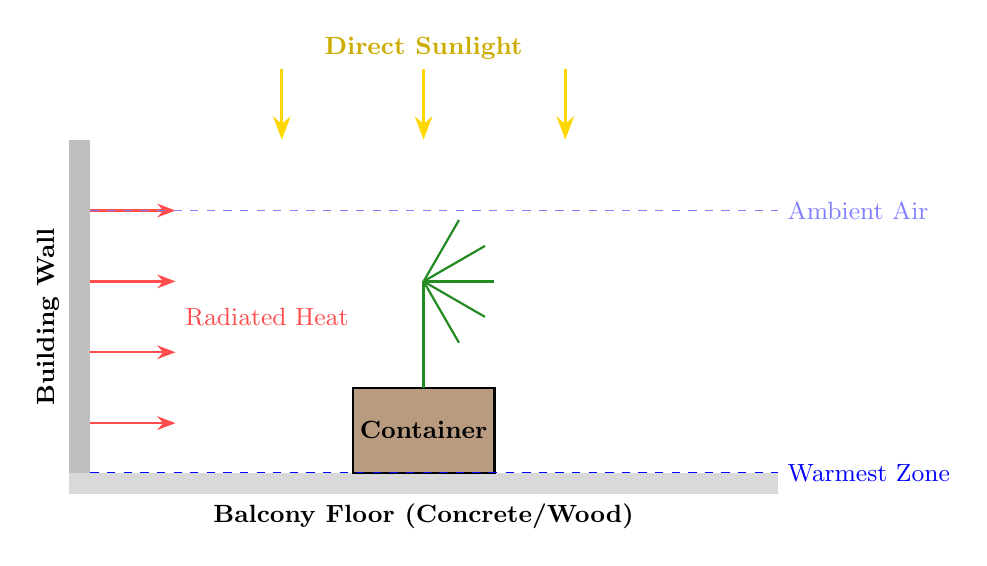
\begin{tikzpicture}[
  remember picture,
  scale=0.9,
  every node/.style={font=\small}
]
  % Balcony structure
  \fill[gray!30] (0,0) rectangle (10,0.3);
  \node[below] at (5,0) {\textbf{Balcony Floor (Concrete/Wood)}};
  
  % Wall
  \fill[gray!50] (0,0.3) rectangle (0.3,5);
  \node[rotate=90] at (-0.3,2.5) {\textbf{Building Wall}};
  
  % Heat radiation arrows
  \foreach \y in {1,2,3,4} {
    \draw[-{Stealth}, red!70, thick] (0.3,\y) -- (1.5,\y);
  }
  \node[right, red!70] at (1.5,2.5) {Radiated Heat};
  
  % Sun arrows
  \foreach \x in {3,5,7} {
    \draw[-{Stealth}, sunlightyellow, very thick] (\x,6) -- (\x,5);
  }
  \node[above, sunlightyellow!80!black] at (5,6) {\textbf{Direct Sunlight}};
  
  % Container
  \fill[soilbrown!60] (4,0.3) rectangle (6,1.5);
  \draw[thick] (4,0.3) rectangle (6,1.5);
  \node at (5,0.9) {\textbf{Container}};
  
  % Plant
  \draw[watermelongreen, very thick] (5,1.5) -- (5,3);
  \foreach \angle in {-60,-30,0,30,60} {
    \draw[watermelongreen, thick] (5,3) -- +(\angle:1);
  }
  
  % Temperature zones
  \draw[dashed, blue] (0.3,0.3) -- (10,0.3);
  \node[right, blue] at (10,0.3) {Warmest Zone};
  
  \draw[dashed, blue!50] (0.3,4) -- (10,4);
  \node[right, blue!50] at (10,4) {Ambient Air};
\end{tikzpicture}

\subsubsection{Advantages}
\begin{itemize}
  \item Thermal mass from adjacent walls and flooring creates warmer microclimate, extending the growing season by 1--2 weeks on both ends
  \item Heat radiated from walls during evening hours helps maintain favorable nighttime temperatures
  \item Ground-level position provides better pollinator access compared to elevated balconies
  \item Wind exposure typically reduced compared to higher floors
  \item Easier access for heavy container management and harvest
\end{itemize}

\subsubsection{Challenges}
\begin{itemize}
  \item Increased pest pressure from ground-dwelling insects and rodents
  \item Potential for fungal issues if airflow is restricted by walls or furniture
  \item Heat stress possible during peak summer if concrete radiates excessive heat
  \item Drainage management critical to prevent water pooling on shared surfaces
  \item Possible shade from overhanging structures or adjacent vegetation
\end{itemize}

\subsection{Critical Temperature Thresholds}

\begin{table}[H]
\centering
\caption{Temperature Requirements for Bradford Watermelons}
\begin{tabular}{@{}p{4.5cm}p{3cm}p{5.5cm}@{}}
\toprule
\textbf{Growth Stage} & \textbf{Temperature} & \textbf{Notes} \\
\midrule
Seed Germination & 70--95\degree F & Optimal: 85\degree F; below 60\degree F = no germination \\
Transplant Soil Temp & 65--70\degree F min & Measure at 4-inch depth \\
Vegetative Growth & 70--85\degree F & Growth slows significantly below 60\degree F \\
Flowering/Pollination & 60--90\degree F & Pollen viability drops above 95\degree F \\
Fruit Development & 70--90\degree F & Consistent temps improve sugar accumulation \\
Danger: Cold Damage & Below 50\degree F & Prolonged exposure causes tissue damage \\
Danger: Heat Stress & Above 95\degree F & Flower drop; reduced fruit set \\
\bottomrule
\end{tabular}
\end{table}

\subsection{Detailed Timeline: Primary Growing Season}

\begin{center}
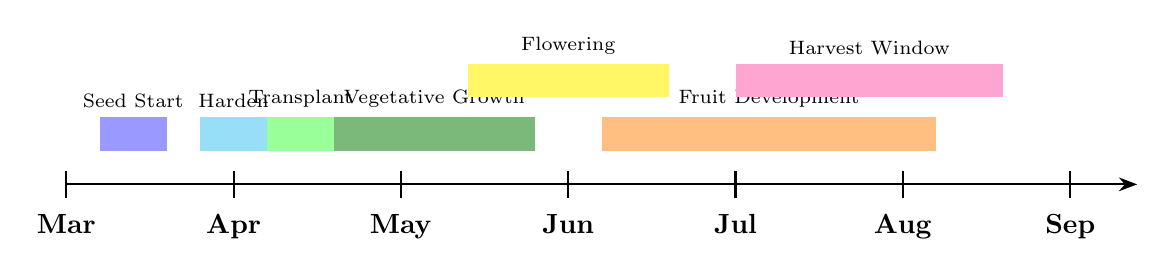
\begin{tikzpicture}[scale=0.85]
  % Timeline base
  \draw[thick, -{Stealth}] (0,0) -- (16,0);
  
  % Month markers
  \foreach \x/\month in {0/Mar, 2.5/Apr, 5/May, 7.5/Jun, 10/Jul, 12.5/Aug, 15/Sep} {
    \draw[thick] (\x,-0.2) -- (\x,0.2);
    \node[below] at (\x,-0.3) {\textbf{\month}};
  }
  
  % Phases with colored bars
  \fill[blue!40] (0.5,0.5) rectangle (1.5,1);
  \node[above, font=\scriptsize] at (1,1) {Seed Start};
  
  \fill[cyan!40] (2,0.5) rectangle (3,1);
  \node[above, font=\scriptsize] at (2.5,1) {Harden};
  
  \fill[green!40] (3,0.5) rectangle (4,1);
  \node[above, font=\scriptsize] at (3.5,1) {Transplant};
  
  \fill[watermelongreen!60] (4,0.5) rectangle (7,1);
  \node[above, font=\scriptsize] at (5.5,1) {Vegetative Growth};
  
  \fill[yellow!60] (6,1.3) rectangle (9,1.8);
  \node[above, font=\scriptsize] at (7.5,1.8) {Flowering};
  
  \fill[orange!50] (8,0.5) rectangle (13,1);
  \node[above, font=\scriptsize] at (10.5,1) {Fruit Development};
  
  \fill[watermelonpink!60] (10,1.3) rectangle (14,1.8);
  \node[above, font=\scriptsize] at (12,1.8) {Harvest Window};
\end{tikzpicture}
\end{center}

\begin{table}[H]
\centering
\caption{Detailed Activity Timeline}
\begin{tabular}{@{}p{3.5cm}p{3cm}p{7cm}@{}}
\toprule
\textbf{Activity} & \textbf{Date Range} & \textbf{Key Actions} \\
\midrule
Seed Starting & Mar 10--20 & Start seeds indoors; maintain 80--85\degree F soil temp \\
Seedling Care & Mar 20--Apr 10 & Provide strong light; maintain moisture; fertilize lightly \\
Hardening Off & Apr 10--20 & Gradual outdoor exposure; 7--10 days minimum \\
Site Preparation & Apr 15--20 & Final container setup; trellis installation; media prep \\
Transplanting & Apr 20--May 5 & Move seedlings to final containers; install protection \\
Early Vegetative & May 1--31 & Establish plants; begin training; monitor for pests \\
Late Vegetative & Jun 1--15 & Vigorous growth; maintain training; adjust feeding \\
Flowering Period & Jun 1--Jul 15 & Hand-pollinate; track flowers; begin fruit selection \\
Fruit Set Decision & Jun 15--Jul 1 & Thin to 1--2 fruits per plant \\
Fruit Development & Jun 20--Aug 15 & Support fruit; manage water; disease prevention \\
Ripening Watch & Jul 15--Aug 30 & Monitor ripeness indicators; reduce watering \\
Harvest & Jul 20--Aug 31 & Harvest at peak ripeness; handle carefully \\
\bottomrule
\end{tabular}
\end{table}

% =============================================================================
% SECTION 3: SCOPE AND SUCCESS CRITERIA
% =============================================================================
\section{Scope and Success Criteria}

\subsection{Project Objective}

Produce ripe, high-quality Bradford watermelons in containers on a ground-level balcony using a combination of vertical training (trellis) and controlled vine management, while maintaining the exceptional fruit quality---size, sweetness, and texture---that defines this heritage variety.

\subsection{Success Metrics}

\begin{table}[H]
\centering
\caption{Quantitative Success Criteria}
\begin{tabular}{@{}p{4cm}p{3cm}p{6.5cm}@{}}
\toprule
\textbf{Metric} & \textbf{Target} & \textbf{Measurement Method} \\
\midrule
Plant Survival Rate & 100\% & Both transplanted seedlings survive to harvest \\
Fruit Set Rate & $\geq$2 fruits & At least one fruit per plant reaches maturity \\
Fruit Size & 12--20 lbs & Scale measurement at harvest \\
Brix Level & $\geq$11\degree & Refractometer reading from flesh sample \\
Days to Harvest & 85--100 days & Calendar tracking from transplant date \\
Plant Health Score & $\geq$7/10 & Weekly visual assessment per rubric \\
\bottomrule
\end{tabular}
\end{table}

\subsection{Realistic Expectations for Container Growing}

\begin{warningbox}
Container growing inherently limits potential compared to in-ground cultivation. Set expectations appropriately: smaller fruit, fewer fruits per plant, and higher maintenance requirements are normal outcomes, not failures.
\end{warningbox}

\begin{itemize}
  \item \textbf{Plant count:} Target \textbf{2 plants} for optimal results. A single plant provides no redundancy; three or more plants compete for limited balcony resources and increase management complexity without proportional yield gains.
  
  \item \textbf{Fruit load:} Thin aggressively to \textbf{1--2 melons per plant}. Attempting more fruits results in smaller, less sweet melons that fail to represent Bradford quality.
  
  \item \textbf{Fruit size:} Expect 12--20 lb melons in containers versus 20--35 lb potential in-ground. This is acceptable; flavor quality should remain high with proper management.
  
  \item \textbf{Season length:} Container plants may decline faster in late season. Prioritize early fruit set and timely harvest over extended production.
\end{itemize}

\subsection{Definition of Done}

A successful Bradford watermelon container project meets all of the following criteria:

\begin{enumerate}
  \item At least one fully ripened fruit harvested from the project
  \item Fruit demonstrates characteristic Bradford sweetness (subjective taste test) or measured Brix $\geq$11\degree
  \item No catastrophic plant loss due to preventable causes (pest infestation, disease, drought stress)
  \item Growing documentation completed for future season improvement
  \item Post-harvest analysis recorded with lessons learned
\end{enumerate}

% =============================================================================
% SECTION 4: RISK CONTROLS
% =============================================================================
\section{Risk Assessment and Mitigation}

\subsection{Risk Matrix}

\begin{table}[H]
\centering
\caption{Risk Assessment Matrix}
\begin{tabular}{@{}p{3.5cm}p{2cm}p{2cm}p{6cm}@{}}
\toprule
\textbf{Risk Category} & \textbf{Likelihood} & \textbf{Impact} & \textbf{Primary Mitigation} \\
\midrule
Pollination failure & Medium & High & Hand-pollination protocol \\
Pest infestation & High & Medium & IPM ladder; early monitoring \\
Fungal disease & Medium & High & Airflow management; soil-line watering \\
Heat stress & Medium & Medium & Afternoon shade; mulching; irrigation \\
Drought stress & Medium & High & Drip irrigation; moisture monitoring \\
Container failure & Low & High & Structural inspection; quality materials \\
Trellis failure & Low & Critical & Proper anchoring; load ratings \\
Rodent damage & Medium & Medium & Physical barriers; elevated fruit \\
Poor fruit quality & Medium & High & Strict thinning; nutrition management \\
Premature frost & Low & High & Weather monitoring; protection ready \\
\bottomrule
\end{tabular}
\end{table}

\subsection{Ground-Level Balcony Specific Risks}

\subsubsection{Increased Pest Pressure}

Ground-level locations experience higher pest populations due to proximity to soil, mulched beds, and vegetation. Key pests include:

\begin{itemize}
  \item \textbf{Cucumber beetles:} Primary vector for bacterial wilt; attracted to cucurbit flowers
  \item \textbf{Aphids:} Rapid reproduction in warm weather; honeydew attracts ants and promotes sooty mold
  \item \textbf{Spider mites:} Thrive in hot, dry conditions common near heat-radiating walls
  \item \textbf{Squash bugs:} Lay eggs on leaf undersides; nymphs cause significant damage
  \item \textbf{Ants:} Farm aphids; may nest in containers; disturb root systems
  \item \textbf{Rodents:} Mice and rats attracted to ripening fruit; can damage vines
\end{itemize}

\subsubsection{Fungal Pressure}

Restricted airflow from walls and railings, combined with Georgia's humidity, creates favorable conditions for fungal pathogens.

\begin{itemize}
  \item \textbf{Powdery mildew:} White patches on leaves; reduces photosynthesis
  \item \textbf{Downy mildew:} Angular lesions; rapid spread in humid conditions
  \item \textbf{Anthracnose:} Fruit and leaf lesions; worse in wet weather
  \item \textbf{Fusarium wilt:} Soil-borne; causes vine collapse
  \item \textbf{Root rot:} From overwatering or poor drainage
\end{itemize}

\subsubsection{Structural Concerns}

\begin{criticalbox}
Ground-level balconies may have weight limits and structural constraints. Verify load capacity before installing heavy containers, water-saturated media, and trellises with fruit load. A single 30-gallon container with saturated media can weigh over 250 lbs.
\end{criticalbox}

\subsection{Comprehensive Mitigation Strategy}

This run book employs a prevention-first approach organized into the following control layers:

\begin{enumerate}
  \item \textbf{Environmental controls:} Container spacing, airflow management, sun exposure optimization
  \item \textbf{Cultural controls:} Soil-line watering, sanitation, proper nutrition, crop rotation (seasonal)
  \item \textbf{Physical controls:} Trellis design, fruit slings, insect netting, rodent barriers
  \item \textbf{Biological controls:} Encourage beneficial insects; avoid broad-spectrum pesticides
  \item \textbf{Chemical controls:} Escalation-based IPM using least-toxic effective treatments
  \item \textbf{Monitoring:} Regular inspection schedule with documented findings
\end{enumerate}

% =============================================================================
% SECTION 5: MATERIALS AND TOOLS
% =============================================================================
\section{Materials and Tools}

This section provides a procurement-ready specification list. Items are categorized by function with minimum and recommended specifications. The recommended tier reflects Bradford-optimized choices for best results.

\subsection{Container System}

\begin{table}[H]
\centering
\caption{Container Specifications}
\begin{tabular}{@{}p{3cm}p{5cm}p{5.5cm}@{}}
\toprule
\textbf{Component} & \textbf{Minimum Spec} & \textbf{Recommended Spec} \\
\midrule
Primary Containers & 2× 20-gallon & 2× 25--30 gallon; fabric grow bags or heavy-duty plastic \\
Material & Any durable material & UV-resistant; light colored to reduce heat absorption \\
Drainage & Holes present & Multiple 1/2-inch holes; elevated on pot feet \\
Pot Feet/Risers & Basic spacers & Adjustable risers; 2--3 inch clearance \\
Catch System & Optional trays & Drainage collection that prevents standing water \\
Surface Protection & None required & Waterproof mat under containers \\
\bottomrule
\end{tabular}
\end{table}

\begin{tipbox}
Fabric grow bags offer excellent drainage and air pruning of roots but dry faster than plastic containers. In Georgia summer heat, plastic containers with proper drainage may be easier to manage for consistent moisture.
\end{tipbox}

\subsection{Trellis System}

\begin{table}[H]
\centering
\caption{Trellis Specifications}
\begin{tabular}{@{}p{3cm}p{5cm}p{5.5cm}@{}}
\toprule
\textbf{Component} & \textbf{Minimum Spec} & \textbf{Recommended Spec} \\
\midrule
Frame Height & 6 ft usable & 7--8 ft total; galvanized conduit or treated lumber \\
Frame Width & 3 ft per plant & 4--5 ft per plant for adequate spread \\
Panel Type & Rigid lattice & Welded wire/cattle panel; 6-inch grid \\
Load Rating & 50 lbs per trellis & 100+ lbs; calculate fruit + vine weight \\
Anchoring & Wall brackets & Wall/floor anchors; railing clamps; guy wires \\
Fasteners & Zip ties & Stainless steel wire; U-bolts; hose clamps \\
Soft Ties & Cloth strips & Velcro plant ties; stretch tie tape \\
\bottomrule
\end{tabular}
\end{table}

\begin{center}
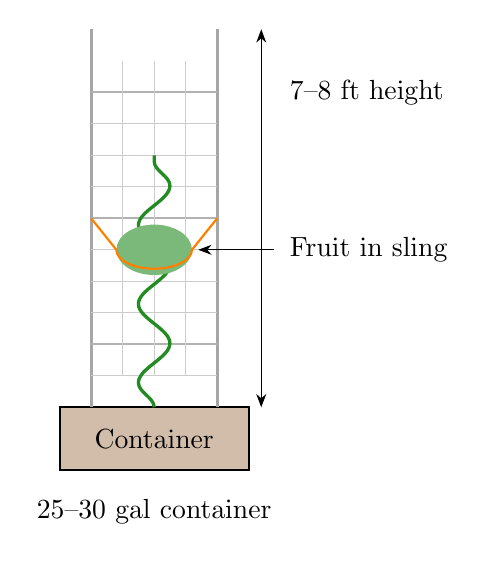
\begin{tikzpicture}[scale=0.8]
  % Container
  \fill[soilbrown!40] (0,0) rectangle (3,1);
  \draw[thick] (0,0) rectangle (3,1);
  \node at (1.5,0.5) {Container};
  
  % Trellis posts
  \draw[very thick, gray!70] (0.5,1) -- (0.5,7);
  \draw[very thick, gray!70] (2.5,1) -- (2.5,7);
  
  % Horizontal supports
  \foreach \y in {2,4,6} {
    \draw[thick, gray!60] (0.5,\y) -- (2.5,\y);
  }
  
  % Grid lines
  \foreach \x in {1,1.5,2} {
    \draw[gray!40] (\x,1.5) -- (\x,6.5);
  }
  \foreach \y in {1.5,2.5,3,3.5,4.5,5,5.5} {
    \draw[gray!40] (0.5,\y) -- (2.5,\y);
  }
  
  % Vine
  \draw[watermelongreen, very thick, decorate, decoration={snake, amplitude=2mm, segment length=10mm}] 
    (1.5,1) -- (1.5,5);
  
  % Fruit with sling
  \fill[watermelongreen!60] (1.5,3.5) ellipse (0.6 and 0.4);
  \draw[orange, thick] (0.9,3.5) arc (180:360:0.6 and 0.3);
  \draw[orange, thick] (0.9,3.5) -- (0.5,4);
  \draw[orange, thick] (2.1,3.5) -- (2.5,4);
  
  % Labels
  \node[right] at (3.5,6) {7--8 ft height};
  \draw[{Stealth}-{Stealth}] (3.2,1) -- (3.2,7);
  
  \node[right] at (3.5,3.5) {Fruit in sling};
  \draw[-{Stealth}] (3.4,3.5) -- (2.2,3.5);
  
  \node[below] at (1.5,-0.3) {25--30 gal container};
\end{tikzpicture}
\captionof{figure}{Trellis Configuration with Fruit Support}
\end{center}

\subsection{Growing Media and Amendments}

\begin{table}[H]
\centering
\caption{Growing Media Specifications}
\begin{tabular}{@{}p{3.5cm}p{4cm}p{6cm}@{}}
\toprule
\textbf{Component} & \textbf{Quantity (2 plants)} & \textbf{Specification} \\
\midrule
Potting Mix & 5--6 cubic ft & High-quality container mix; avoid ``garden soil'' \\
Compost & 1--1.5 cubic ft & Well-aged; 15--20\% of total volume \\
Perlite/Pumice & 0.5--1 cubic ft & If mix compacts; 10--15\% addition \\
Worm Castings & 1--2 quarts & Optional; for early vigor \\
Mulch & 0.5 cubic ft & Straw or shredded leaves; 2--3 inch layer \\
\bottomrule
\end{tabular}
\end{table}

\subsubsection{Media Preparation Recipe}

\begin{procedurebox}[Optimal Container Media Mix]
\begin{enumerate}
  \item Base: 70\% quality potting mix (peat or coir based)
  \item Add: 20\% finished compost
  \item Add: 10\% perlite (if mix feels dense)
  \item Optional: 1 cup worm castings per container
  \item Mix thoroughly in large tub or tarp
  \item Pre-moisten before filling containers
  \item Fill containers to within 2 inches of rim
  \item Allow to settle 24--48 hours before transplanting
\end{enumerate}
\end{procedurebox}

\subsection{Fertilizers and Nutrition}

\begin{table}[H]
\centering
\caption{Fertilizer Program Components}
\begin{tabular}{@{}p{3.5cm}p{3.5cm}p{6.5cm}@{}}
\toprule
\textbf{Product Type} & \textbf{When Used} & \textbf{Recommended Analysis} \\
\midrule
Balanced Granular & At planting & 10-10-10 or 14-14-14 slow-release \\
Vegetative Liquid & Weeks 1--4 & Fish emulsion (5-1-1) or balanced (10-10-10) \\
Transition Feed & Weeks 4--6 & 5-10-10 or similar reduced nitrogen \\
Fruiting Liquid & Weeks 6+ & 4-8-12 or tomato/pepper fertilizer \\
Calcium Source & Throughout & Calcium nitrate or gypsum for fruit quality \\
Micronutrients & Monthly & Kelp extract or complete micronutrient blend \\
\bottomrule
\end{tabular}
\end{table}

\begin{warningbox}
Excess nitrogen during fruiting causes ``all vine, no fruit'' syndrome and reduces sugar content in developing melons. Transition to low-nitrogen, high-potassium feeding once flowering begins.
\end{warningbox}

\subsection{Irrigation System}

\begin{table}[H]
\centering
\caption{Irrigation Options}
\begin{tabular}{@{}p{3cm}p{4cm}p{6.5cm}@{}}
\toprule
\textbf{Method} & \textbf{Minimum Setup} & \textbf{Recommended Setup} \\
\midrule
Manual & Watering can; hose access & Hose with adjustable wand; shutoff valve \\
Drip System & Basic drip emitters & Timer-controlled; 2 GPH emitters; 2 per pot \\
Soaker Option & Soaker hose coiled in pot & Pressure-regulated soaker with timer \\
Monitoring & Finger test (2--3 in depth) & Soil moisture meter; multiple readings \\
\bottomrule
\end{tabular}
\end{table}

\subsection{Pollination Kit}

\begin{itemize}
  \item Small artist paintbrushes (2--3 soft bristle brushes)
  \item Cotton swabs (backup method)
  \item Plant tags and permanent marker for dating pollinated flowers
  \item Small notebook for pollination log
  \item Hand lens or magnifying glass for flower inspection
\end{itemize}

\subsection{Monitoring and IPM Kit}

\begin{table}[H]
\centering
\caption{Pest Management Supplies}
\begin{tabular}{@{}p{4cm}p{4cm}p{5.5cm}@{}}
\toprule
\textbf{Category} & \textbf{Minimum} & \textbf{Recommended} \\
\midrule
Monitoring & Yellow sticky cards (6+) & Sticky cards + hand lens + ID guide \\
Physical Barriers & --- & Insect netting; hardware cloth \\
Soft Treatments & Insecticidal soap & Soap + neem oil + horticultural oil \\
Application & Spray bottle & Pump sprayer (1--2 gal); dedicated \\
Sanitation & Trash bags & Bags + rubbing alcohol + clean cloths \\
\bottomrule
\end{tabular}
\end{table}

\subsection{Tools Checklist}

\begin{multicols}{2}
\textbf{Container and Media:}
\begin{itemize}[nosep]
  \item Large mixing tub or tarp
  \item Hand trowel
  \item Measuring cups for fertilizer
  \item Watering wand or can
\end{itemize}

\textbf{Trellis Installation:}
\begin{itemize}[nosep]
  \item Drill/driver with bits
  \item Level (torpedo or 2-ft)
  \item Tape measure
  \item Wire cutters
  \item Pliers
  \item Work gloves
  \item Safety glasses
\end{itemize}

\columnbreak

\textbf{Plant Care:}
\begin{itemize}[nosep]
  \item Bypass pruners (clean, sharp)
  \item Plant ties and clips
  \item Soil thermometer
  \item Moisture meter
  \item Refractometer (optional, for Brix)
\end{itemize}

\textbf{Harvest:}
\begin{itemize}[nosep]
  \item Sharp knife or pruners
  \item Scale (for weighing fruit)
  \item Soft padding for transport
\end{itemize}
\end{multicols}

\subsection{Procurement Sources}

\begin{infobox}
\textbf{Bradford watermelon seeds} are available exclusively from Nat Bradford's official source or authorized seed companies carrying the Bradford Family line. Verify authenticity before purchasing, as mislabeled seeds are common for heritage varieties.

Recommended supplier: Bradford Watermelons (bradfordwatermelons.com) or Southern Exposure Seed Exchange.
\end{infobox}

% =============================================================================
% SECTION 6: BALCONY LAYOUT
% =============================================================================
\section{Balcony Layout and Spacing}

\subsection{Standard Layout (12×11 ft Balcony)}

\begin{center}
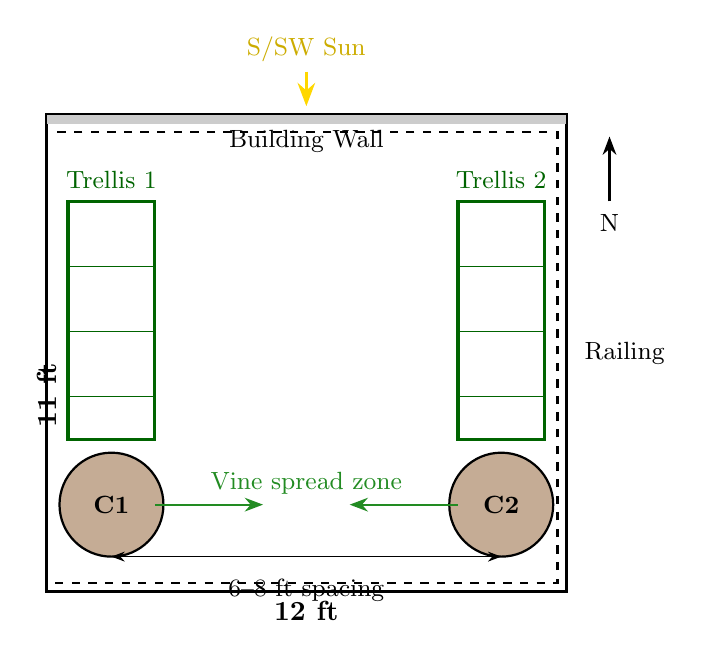
\begin{tikzpicture}[scale=0.55]
  % Balcony outline
  \draw[very thick] (0,0) rectangle (12,11);
  \node[below] at (6,0) {\textbf{12 ft}};
  \node[left, rotate=90] at (0,5.5) {\textbf{11 ft}};
  
  % Building wall
  \fill[gray!40] (0,10.8) rectangle (12,11);
  \node at (6,10.4) {\small Building Wall};
  
  % Railing
  \draw[thick, dashed] (0.2,0.2) -- (11.8,0.2) -- (11.8,10.6) -- (0.2,10.6);
  \node[right] at (12.2,5.5) {\small Railing};
  
  % Container 1
  \fill[soilbrown!50] (1.5,2) circle (1.2);
  \draw[thick] (1.5,2) circle (1.2);
  \node at (1.5,2) {\small \textbf{C1}};
  
  % Container 2
  \fill[soilbrown!50] (10.5,2) circle (1.2);
  \draw[thick] (10.5,2) circle (1.2);
  \node at (10.5,2) {\small \textbf{C2}};
  
  % Trellis 1
  \draw[very thick, darkgreen] (0.5,3.5) rectangle (2.5,9);
  \draw[darkgreen] (0.5,4.5) -- (2.5,4.5);
  \draw[darkgreen] (0.5,6) -- (2.5,6);
  \draw[darkgreen] (0.5,7.5) -- (2.5,7.5);
  \node[darkgreen] at (1.5,9.5) {\small Trellis 1};
  
  % Trellis 2
  \draw[very thick, darkgreen] (9.5,3.5) rectangle (11.5,9);
  \draw[darkgreen] (9.5,4.5) -- (11.5,4.5);
  \draw[darkgreen] (9.5,6) -- (11.5,6);
  \draw[darkgreen] (9.5,7.5) -- (11.5,7.5);
  \node[darkgreen] at (10.5,9.5) {\small Trellis 2};
  
  % Vine spread indication
  \draw[watermelongreen, thick, -{Stealth}] (2.5,2) -- (5,2);
  \draw[watermelongreen, thick, -{Stealth}] (9.5,2) -- (7,2);
  \node[watermelongreen] at (6,2.5) {\small Vine spread zone};
  
  % Spacing annotation
  \draw[{Stealth}-{Stealth}] (1.5,0.8) -- (10.5,0.8);
  \node[below] at (6,0.5) {\small 6--8 ft spacing};
  
  % Sun direction
  \draw[sunlightyellow, very thick, -{Stealth}] (6,12) -- (6,11.2);
  \node[above, sunlightyellow!80!black] at (6,12) {\small S/SW Sun};
  
  % North arrow
  \draw[thick, -{Stealth}] (13,9) -- (13,10.5);
  \node at (13,8.5) {\small N};
\end{tikzpicture}
\captionof{figure}{Recommended Balcony Layout---Two-Plant Configuration}
\end{center}

\subsection{Spacing Guidelines}

\begin{itemize}
  \item \textbf{Container separation:} 6--8 ft minimum between container centers. Corner placement maximizes usable balcony space while maintaining separation.
  
  \item \textbf{Wall clearance:} Position trellises 6--12 inches from walls to allow air circulation behind vines and prevent heat damage from direct wall contact.
  
  \item \textbf{Railing clearance:} Keep containers and vine growth at least 12 inches inside railings for wind protection and to avoid overhanging shared spaces.
  
  \item \textbf{Traffic path:} Maintain 3--4 ft clear path through center for access, watering, and harvest operations.
  
  \item \textbf{Sun optimization:} Orient trellises perpendicular to primary sun direction (typically south-facing in Atlanta area) to maximize light exposure on both sides of vine growth.
\end{itemize}

\subsection{Alternative Layouts}

\subsubsection{Single Plant (Minimum Viable)}

For smaller balconies (under 100 sq ft), a single plant in a 30-gallon container with a 4-ft wide trellis can produce 1--2 quality melons. This configuration eliminates redundancy but reduces management complexity.

\subsubsection{Three-Plant Layout (Advanced)}

Only attempt three plants if:
\begin{itemize}
  \item Balcony exceeds 150 sq ft
  \item Containers can be spaced 5+ ft apart
  \item Aggressive fruit thinning to 1 melon per plant is acceptable
  \item Water and fertilizer capacity can handle 50\% increased demand
\end{itemize}

% =============================================================================
% SECTION 7: OPERATING PROCEDURES
% =============================================================================
\section{Phase-by-Phase Operating Procedures}

\subsection{Phase 1: Seed Starting (March 10--20)}

\subsubsection{Objective}
Germinate Bradford watermelon seeds indoors to produce stocky, healthy seedlings ready for hardening and transplant.

\subsubsection{Materials Required}
\begin{itemize}
  \item Bradford watermelon seeds (3--4 seeds for 2 plants; allows selection)
  \item Seed starting mix (sterile, fine-textured)
  \item 3--4 inch pots or cell trays
  \item Heat mat with thermostat
  \item Grow lights or bright south-facing window
  \item Spray bottle for misting
  \item Thermometer for monitoring soil temperature
\end{itemize}

\subsubsection{Procedure}

\begin{procedurebox}[Seed Starting Protocol]
\begin{enumerate}
  \item \textbf{Prepare containers:} Fill pots with pre-moistened seed starting mix to within 1/2 inch of rim. Mix should be damp but not waterlogged (squeeze test: a few drops when compressed).
  
  \item \textbf{Plant seeds:} Place 1--2 seeds per pot, 1 inch deep. Cover lightly and firm gently. Label with date and variety.
  
  \item \textbf{Provide bottom heat:} Place on heat mat set to 80--85\degree F. Monitor actual soil temperature with probe thermometer. Adjust as needed.
  
  \item \textbf{Maintain moisture:} Cover loosely with humidity dome or plastic wrap until germination. Mist surface if drying occurs. Remove cover at first sign of emergence.
  
  \item \textbf{Germination watch:} Expect emergence in 4--7 days at optimal temperature. Germination may take 10--14 days if temperatures fluctuate.
  
  \item \textbf{Light provision:} Upon emergence, provide 14--16 hours of strong light daily. Position grow lights 2--4 inches above seedlings. Rotate pots if using window light to prevent leaning.
  
  \item \textbf{Temperature management:} After germination, reduce to 70--75\degree F daytime, 60--65\degree F nighttime to encourage stocky growth. Remove heat mat once established.
  
  \item \textbf{Thinning:} If multiple seeds germinate per pot, snip weaker seedling at soil line when first true leaf appears. Do not pull to avoid root disturbance.
  
  \item \textbf{Watering:} Water when surface begins to dry. Avoid soggy conditions which promote damping off. Bottom watering preferred.
  
  \item \textbf{Feeding:} Begin dilute fertilizer (1/4 strength balanced liquid) when first true leaves are fully expanded, approximately 10--14 days after emergence.
\end{enumerate}
\end{procedurebox}

\subsubsection{Quality Gate}
Seedlings are ready to advance when they exhibit:
\begin{itemize}
  \item 2--3 true leaves fully expanded
  \item Stocky stem (not leggy or stretched)
  \item Healthy green color without yellowing
  \item White root tips visible at drainage holes (not circling or matted)
  \item No signs of disease or pest damage
\end{itemize}

\subsection{Phase 2: Hardening Off (April 10--20)}

\subsubsection{Objective}
Acclimate seedlings to outdoor conditions to prevent transplant shock.

\subsubsection{Procedure}

\begin{table}[H]
\centering
\caption{Hardening Off Schedule}
\begin{tabular}{@{}clp{7cm}@{}}
\toprule
\textbf{Day} & \textbf{Duration} & \textbf{Conditions} \\
\midrule
1--2 & 2 hours & Shaded, protected location; no direct sun or wind \\
3--4 & 4 hours & Partial shade; light breeze acceptable \\
5--6 & 6 hours & Morning sun (2 hours direct); afternoon shade \\
7--8 & 8 hours & Half-day sun; return indoors at night \\
9--10 & Full day & Full outdoor conditions; overnight outside if $>$55\degree F \\
\bottomrule
\end{tabular}
\end{table}

\begin{warningbox}
Never expose unhardened seedlings to direct midday sun, strong wind, or temperatures below 50\degree F. A single day of stress can set back transplant readiness by a week or more.
\end{warningbox}

\subsection{Phase 3: Site Preparation and Transplanting (April 15--May 5)}

\subsubsection{Pre-Transplant Site Checklist}

Complete all site preparation during the final week of hardening off:

\begin{itemize}
  \item[\cb] Containers positioned and filled with prepared media
  \item[\cb] Media pre-moistened and settled (24--48 hours)
  \item[\cb] Slow-release fertilizer incorporated per label rate
  \item[\cb] Trellis fully assembled and anchored (load-tested)
  \item[\cb] Irrigation system installed and tested
  \item[\cb] Mulch materials staged (apply after soil warms)
  \item[\cb] Pest monitoring cards deployed
  \item[\cb] Row cover or insect netting ready if needed
\end{itemize}

\subsubsection{Transplanting Protocol}

\begin{procedurebox}[Transplant Day Procedure]
\textbf{Timing:} Late afternoon or overcast day preferred to reduce transplant stress.

\begin{enumerate}
  \item Water seedlings thoroughly 1--2 hours before transplanting.
  
  \item Verify soil temperature in containers: minimum 65\degree F at 4-inch depth.
  
  \item Create planting hole slightly larger than root ball.
  
  \item Gently remove seedling from pot. Support root ball; minimize disturbance.
  
  \item Place seedling at same depth as grown (do not bury stem).
  
  \item Backfill and firm gently to eliminate air pockets.
  
  \item Water in thoroughly with dilute transplant fertilizer (high phosphorus) or plain water.
  
  \item Install plant collar or cutworm barrier around stem base.
  
  \item Apply mulch 2--3 inches deep, keeping 2-inch clearance from stem.
  
  \item Install temporary shade cover if hot sun expected within 48 hours.
  
  \item Secure main stem loosely to first trellis support.
  
  \item Record transplant date in growing log.
\end{enumerate}
\end{procedurebox}

\subsubsection{Post-Transplant Monitoring (First 7 Days)}

\begin{itemize}
  \item Check daily for wilting; water as needed to maintain even moisture
  \item Watch for cutworm damage (stem severed at soil line)
  \item Monitor for transplant shock symptoms: severe wilting, leaf drop, failure to establish
  \item Protect from unexpected cold snaps with frost cloth or milk jug cloches
  \item Expect some initial stress; recovery within 5--7 days is normal
\end{itemize}

\textbf{Pass criteria:} New leaf growth visible within 7 days; no sustained wilting beyond afternoon hours; plant anchored and upright.

\subsection{Phase 4: Vegetative Growth and Training (Weeks 1--5)}

\subsubsection{Daily Operations (5--10 minutes)}

\begin{itemize}
  \item \textbf{Moisture check:} Insert finger or probe 2--3 inches into media. Water if dry at that depth. Water at soil line; keep foliage dry.
  
  \item \textbf{Visual scan:} Check leaf surfaces (both sides) for pest presence, unusual spots, or wilting patterns.
  
  \item \textbf{Drainage confirmation:} Verify water exits freely; no standing water in trays.
\end{itemize}

\subsubsection{Twice Weekly Operations (10--15 minutes)}

\begin{itemize}
  \item \textbf{Vine training:} Guide main leader up trellis using soft ties. Secure every 8--12 inches. Ties should be loose enough to allow stem expansion.
  
  \item \textbf{Lateral management:} Allow 2--3 strong lateral branches to develop. Remove weak or crowded laterals while small.
  
  \item \textbf{Tie inspection:} Check all ties for tightness; replace any that are constricting.
\end{itemize}

\subsubsection{Weekly Operations (15--20 minutes)}

\begin{itemize}
  \item \textbf{Feeding:} Apply liquid fertilizer per schedule (balanced formula, weeks 1--4).
  
  \item \textbf{Sticky card review:} Inspect monitoring cards for pest trends. Record findings.
  
  \item \textbf{Underside leaf inspection:} Examine undersides of older leaves for mites, aphids, or early disease signs.
  
  \item \textbf{Sanitation:} Remove fallen leaves, spent flowers, and debris from container surface.
  
  \item \textbf{Growth logging:} Measure and record vine length; note plant health observations.
\end{itemize}

\subsubsection{Vine Training Diagram}

\begin{center}
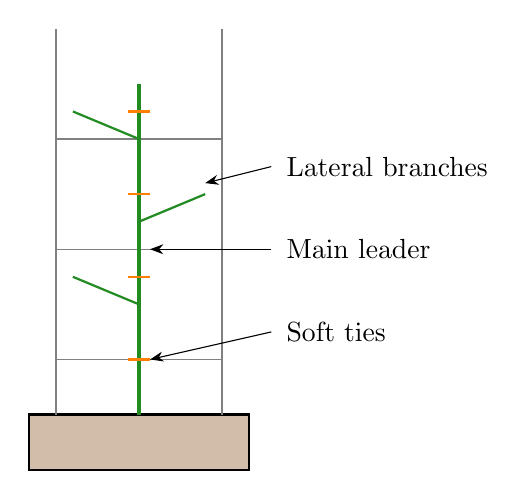
\begin{tikzpicture}[scale=0.7]
  % Container
  \fill[soilbrown!40] (0,0) rectangle (4,1);
  \draw[thick] (0,0) rectangle (4,1);
  
  % Trellis
  \draw[thick, gray] (0.5,1) -- (0.5,8);
  \draw[thick, gray] (3.5,1) -- (3.5,8);
  \foreach \y in {2,4,6} {
    \draw[gray] (0.5,\y) -- (3.5,\y);
  }
  
  % Main vine
  \draw[watermelongreen, very thick] (2,1) -- (2,7);
  
  % Laterals
  \draw[watermelongreen, thick] (2,3) -- (0.8,3.5);
  \draw[watermelongreen, thick] (2,4.5) -- (3.2,5);
  \draw[watermelongreen, thick] (2,6) -- (0.8,6.5);
  
  % Ties
  \foreach \y in {2,3.5,5,6.5} {
    \draw[orange, thick] (1.8,\y) -- (2.2,\y);
  }
  
  % Labels
  \node[right] at (4.5,4) {Main leader};
  \draw[-{Stealth}] (4.4,4) -- (2.2,4);
  
  \node[right] at (4.5,5.5) {Lateral branches};
  \draw[-{Stealth}] (4.4,5.5) -- (3.2,5.2);
  
  \node[right] at (4.5,2.5) {Soft ties};
  \draw[-{Stealth}] (4.4,2.5) -- (2.2,2);
\end{tikzpicture}
\captionof{figure}{Vertical Vine Training Pattern}
\end{center}

\subsection{Phase 5: Flowering and Pollination (Weeks 4--7)}

\subsubsection{Flower Identification}

\begin{center}
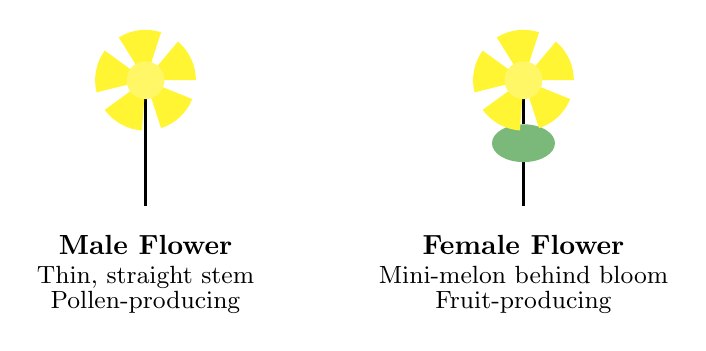
\begin{tikzpicture}[scale=0.8]
  % Male flower
  \begin{scope}[shift={(0,0)}]
    \draw[thick] (0,0) -- (0,2);
    \foreach \angle in {0,72,144,216,288} {
      \fill[yellow!80] (0,2) -- ++(\angle:0.8) arc (\angle:\angle+50:0.8) -- cycle;
    }
    \fill[yellow!60] (0,2) circle (0.3);
    \node[below] at (0,-0.3) {\textbf{Male Flower}};
    \node[below] at (0,-0.8) {\small Thin, straight stem};
    \node[below] at (0,-1.2) {\small Pollen-producing};
  \end{scope}
  
  % Female flower
  \begin{scope}[shift={(6,0)}]
    \draw[thick] (0,0) -- (0,1);
    \fill[watermelongreen!60] (0,1) ellipse (0.5 and 0.3);
    \draw[thick] (0,1.3) -- (0,2);
    \foreach \angle in {0,72,144,216,288} {
      \fill[yellow!80] (0,2) -- ++(\angle:0.8) arc (\angle:\angle+50:0.8) -- cycle;
    }
    \fill[yellow!60] (0,2) circle (0.3);
    \node[below] at (0,-0.3) {\textbf{Female Flower}};
    \node[below] at (0,-0.8) {\small Mini-melon behind bloom};
    \node[below] at (0,-1.2) {\small Fruit-producing};
  \end{scope}
\end{tikzpicture}
\captionof{figure}{Male vs. Female Flower Identification}
\end{center}

\subsubsection{Hand-Pollination Protocol}

\begin{procedurebox}[Morning Pollination Procedure (6--10 AM)]
\begin{enumerate}
  \item Identify newly opened female flowers (look for swelling at base).
  
  \item Locate fresh male flowers on the same or nearby plant.
  
  \item Option A (preferred): Remove male flower, peel back petals to expose anther, touch directly to female stigma with gentle rotating motion.
  
  \item Option B: Use soft paintbrush to collect yellow pollen from male flower, transfer to center of female flower with dabbing motion.
  
  \item Ensure pollen is visible on stigma surface after transfer.
  
  \item Tag pollinated flower with date using plant tag or marker.
  
  \item Repeat daily for 7--10 days during peak flowering to ensure adequate fruit set.
  
  \item Record all pollination attempts in log.
\end{enumerate}
\end{procedurebox}

\begin{tipbox}
Flowers are most receptive in early morning. Pollen viability decreases rapidly as temperatures rise above 90\degree F. On hot days, complete pollination before 9 AM for best results.
\end{tipbox}

\subsubsection{Fruit Set Decision}

Once fruit begins developing (golf ball size or larger, approximately 7--10 days after successful pollination):

\begin{enumerate}
  \item Assess total developing fruit count per plant
  \item Select 1--2 healthiest, best-positioned fruits to keep
  \item Remove all other developing fruits by cutting stem cleanly
  \item Concentrate remaining plant resources on selected fruits
\end{enumerate}

\begin{criticalbox}
Failing to thin fruit is the most common cause of poor quality in container watermelons. Be ruthless in selection. It is better to have one excellent 15 lb melon than three mediocre 5 lb melons.
\end{criticalbox}

\subsection{Phase 6: Fruit Development and Support (Weeks 6--12)}

\subsubsection{Sling Installation}

\begin{procedurebox}[Fruit Sling Installation]
\textbf{Timing:} When fruit reaches softball size (approximately 4--5 inches diameter).

\begin{enumerate}
  \item Select sling material: mesh produce bag, cloth strip, or commercial melon sling.
  
  \item Create cradle that supports fruit from below without squeezing.
  
  \item Attach sling to trellis structure (not to vine or fruit stem).
  
  \item Position so fruit weight is transferred to trellis, relieving stem stress.
  
  \item Verify sling allows air circulation around fruit.
  
  \item Check and adjust weekly as fruit grows; expand or replace as needed.
  
  \item Never let fruit hang unsupported once larger than softball size.
\end{enumerate}
\end{procedurebox}

\subsubsection{Water Management During Fruit Development}

\begin{table}[H]
\centering
\caption{Irrigation Adjustment Schedule}
\begin{tabular}{@{}p{4cm}p{4.5cm}p{5cm}@{}}
\toprule
\textbf{Stage} & \textbf{Moisture Target} & \textbf{Notes} \\
\midrule
Early fruit (weeks 6--8) & Consistently moist & Critical period; avoid drought stress \\
Mid-development (weeks 8--10) & Even moisture & Maintain steady conditions \\
Pre-ripening (weeks 10--12) & Reduce by 25--30\% & Concentrates sugars; reduces splitting \\
Final week & Minimal & Light water only if severely wilting \\
\bottomrule
\end{tabular}
\end{table}

\subsubsection{Nutrition During Fruiting}

\begin{itemize}
  \item Switch to low-nitrogen, high-potassium fertilizer once fruit is set
  \item Continue calcium supplementation to prevent blossom end rot
  \item Reduce feeding frequency to every 10--14 days during active fruit growth
  \item Discontinue all fertilizer 2 weeks before expected harvest
\end{itemize}

\subsection{Phase 7: Ripening and Harvest}

\subsubsection{Ripeness Indicators}

Bradford watermelons exhibit several indicators when approaching harvest readiness. Multiple indicators should be present before harvest.

\begin{table}[H]
\centering
\caption{Ripeness Assessment Criteria}
\begin{tabular}{@{}p{3.5cm}p{4cm}p{6cm}@{}}
\toprule
\textbf{Indicator} & \textbf{Unripe Sign} & \textbf{Ripe Sign} \\
\midrule
Tendril nearest fruit & Green, curly & Brown, dried, withered \\
Ground/belly spot & White or pale green & Creamy yellow to butter yellow \\
Rind surface & Shiny, bright & Slightly dull, matte finish \\
Rind hardness & Soft, easily scratched & Hard, resists fingernail \\
Sound when tapped & High-pitched, metallic & Deep, hollow ``thunk'' \\
Days from pollination & Less than 35 days & 35--45 days (Bradford specific) \\
\bottomrule
\end{tabular}
\end{table}

\begin{tipbox}
The dried tendril is the most reliable single indicator for Bradford watermelons. When the tendril opposite the fruit stem is completely brown and dried, the fruit is likely ready. Combine with ground spot color for highest accuracy.
\end{tipbox}

\subsubsection{Harvest Procedure}

\begin{procedurebox}[Harvest Protocol]
\begin{enumerate}
  \item Verify multiple ripeness indicators are present.
  
  \item Harvest in early morning when fruit is coolest.
  
  \item Remove sling carefully; support fruit weight manually.
  
  \item Cut stem with clean, sharp pruners or knife, leaving 2 inches of stem attached.
  
  \item Do not pull or twist fruit; this damages stem attachment point.
  
  \item Handle gently; Bradford rinds are thin and bruise easily.
  
  \item Place on soft surface immediately; avoid dropping or rolling.
  
  \item Record harvest date, fruit weight, and visual quality notes.
  
  \item Store at room temperature for best flavor (1--2 weeks maximum).
  
  \item Refrigerate only after cutting; consume cut melon within 3--5 days.
\end{enumerate}
\end{procedurebox}

% =============================================================================
% SECTION 8: ROUTINE CHECKLISTS
% =============================================================================
\section{Routine Maintenance Checklists}

\subsection{Daily Checklist (5 Minutes)}

\begin{itemize}
  \item[\cb] Soil moisture check (2--3 inch depth)
  \item[\cb] Visual scan for wilting or stress
  \item[\cb] Pest and disease quick check (tops and undersides of leaves)
  \item[\cb] Confirm drainage (no standing water)
  \item[\cb] Check weather forecast for alerts
\end{itemize}

\subsection{Twice-Weekly Checklist (10--15 Minutes)}

\begin{itemize}
  \item[\cb] Vine training and tie adjustment
  \item[\cb] Sling inspection and adjustment (during fruit phase)
  \item[\cb] Remove severely damaged or diseased foliage
  \item[\cb] Check trellis stability
  \item[\cb] Hand-pollinate (during flowering phase)
\end{itemize}

\subsection{Weekly Checklist (20--30 Minutes)}

\begin{itemize}
  \item[\cb] Fertilizer application per schedule
  \item[\cb] Deep inspection: undersides of all leaves
  \item[\cb] Sticky card review and replacement if needed
  \item[\cb] Container surface sanitation (remove debris)
  \item[\cb] Update growing log with measurements and observations
  \item[\cb] Review and adjust irrigation timer/schedule
  \item[\cb] Mulch depth check; replenish if needed
\end{itemize}

\subsection{Monthly Checklist}

\begin{itemize}
  \item[\cb] Soil pH test (target 6.0--6.8)
  \item[\cb] Review overall plant health trend
  \item[\cb] Assess progress against timeline
  \item[\cb] Clean and sanitize pruners and tools
  \item[\cb] Restock supplies as needed
  \item[\cb] Photo documentation for season record
\end{itemize}

% =============================================================================
% SECTION 9: NUTRIENT MANAGEMENT
% =============================================================================
\section{Nutrient Management Program}

\subsection{Feeding Schedule Overview}

\begin{center}
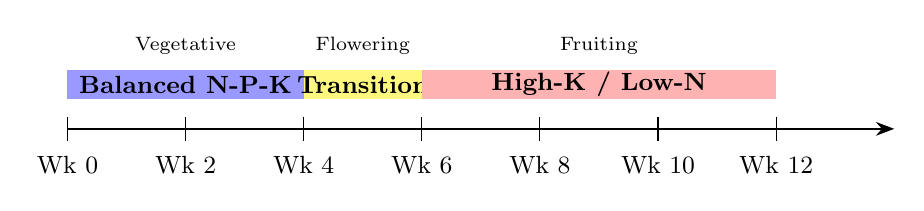
\begin{tikzpicture}[scale=0.75]
  % Timeline
  \draw[thick, -{Stealth}] (0,0) -- (14,0);
  \foreach \x/\label in {0/Wk 0, 2/Wk 2, 4/Wk 4, 6/Wk 6, 8/Wk 8, 10/Wk 10, 12/Wk 12} {
    \draw (\x,-0.2) -- (\x,0.2);
    \node[below] at (\x,-0.3) {\small\label};
  }
  
  % Phase bars
  \fill[blue!40] (0,0.5) rectangle (4,1);
  \node at (2,0.75) {\small\textbf{Balanced N-P-K}};
  
  \fill[yellow!50] (4,0.5) rectangle (6,1);
  \node at (5,0.75) {\small\textbf{Transition}};
  
  \fill[red!30] (6,0.5) rectangle (12,1);
  \node at (9,0.75) {\small\textbf{High-K / Low-N}};
  
  % Annotations
  \node[above] at (2,1.1) {\scriptsize Vegetative};
  \node[above] at (5,1.1) {\scriptsize Flowering};
  \node[above] at (9,1.1) {\scriptsize Fruiting};
\end{tikzpicture}
\end{center}

\subsection{Detailed Feeding Protocol}

\begin{table}[H]
\centering
\caption{Weekly Fertilizer Application Schedule}
\begin{tabular}{@{}clll@{}}
\toprule
\textbf{Week} & \textbf{Product Type} & \textbf{Rate} & \textbf{Notes} \\
\midrule
0 (transplant) & Transplant solution & 1/2 strength & High phosphorus; root establishment \\
1 & Balanced liquid & 1/2 strength & Begin regular feeding \\
2 & Balanced liquid & Full strength & Every 7 days \\
3 & Balanced liquid & Full strength & Monitor for vigorous growth \\
4 & Transition formula & Full strength & Begin nitrogen reduction \\
5 & Low-N formula & Full strength & Flowering support \\
6--8 & Fruiting formula & Full strength & Every 10--14 days \\
9--10 & Fruiting formula & 1/2 strength & Reduce frequency \\
11--12 & None & --- & Discontinue 2 weeks before harvest \\
\bottomrule
\end{tabular}
\end{table}

\subsection{Deficiency Identification}

\begin{table}[H]
\centering
\caption{Common Nutrient Deficiency Symptoms}
\begin{tabular}{@{}p{2.5cm}p{5cm}p{6cm}@{}}
\toprule
\textbf{Nutrient} & \textbf{Symptoms} & \textbf{Correction} \\
\midrule
Nitrogen (N) & Pale green/yellow older leaves; stunted growth & Increase balanced fertilizer; fish emulsion \\
Phosphorus (P) & Purple tinge to leaves; poor root development & Bone meal; high-P transplant fertilizer \\
Potassium (K) & Brown leaf edges; poor fruit quality & Potassium sulfate; increase fruiting fertilizer \\
Calcium (Ca) & Blossom end rot; distorted new growth & Calcium nitrate; gypsum application \\
Magnesium (Mg) & Interveinal yellowing on older leaves & Epsom salt foliar spray (1 tbsp/gallon) \\
Iron (Fe) & Interveinal yellowing on new leaves & Chelated iron; check soil pH \\
\bottomrule
\end{tabular}
\end{table}

% =============================================================================
% SECTION 10: IPM
% =============================================================================
\section{Integrated Pest and Disease Management}

\subsection{Monitoring Protocol}

Effective IPM begins with early detection. Implement the following monitoring schedule:

\begin{itemize}
  \item \textbf{Daily visual scan:} Quick check of plant appearance, obvious pests
  \item \textbf{Twice weekly detailed inspection:} Examine undersides of leaves, stem junctions, new growth
  \item \textbf{Weekly sticky card review:} Identify trapped insects; note trends
  \item \textbf{Record all observations:} Date, pest type, location, severity, action taken
\end{itemize}

\subsection{Common Pests}

\begin{table}[H]
\centering
\caption{Pest Identification and Response}
\begin{tabular}{@{}p{2.5cm}p{4cm}p{7cm}@{}}
\toprule
\textbf{Pest} & \textbf{Identification} & \textbf{Response} \\
\midrule
Aphids & Small, soft-bodied clusters; honeydew residue & Water jet; insecticidal soap; neem oil \\
Spider mites & Stippling; fine webbing; hot/dry conditions & Increase humidity; miticide; neem oil \\
Cucumber beetles & Striped or spotted; 1/4 inch beetles & Hand-pick; row cover; pyrethrin if severe \\
Squash bugs & Gray-brown; shield-shaped; eggs on leaves & Hand-pick; destroy eggs; insecticidal soap \\
Whiteflies & Tiny white flies; clouds when disturbed & Yellow sticky traps; insecticidal soap \\
Ants & Trailing to aphid colonies & Bait stations; barrier treatments; remove aphids \\
\bottomrule
\end{tabular}
\end{table}

\subsection{Common Diseases}

\begin{table}[H]
\centering
\caption{Disease Identification and Response}
\begin{tabular}{@{}p{2.5cm}p{4cm}p{7cm}@{}}
\toprule
\textbf{Disease} & \textbf{Identification} & \textbf{Response} \\
\midrule
Powdery mildew & White powdery coating on leaves & Improve airflow; remove affected leaves; fungicide \\
Downy mildew & Angular yellow lesions; fuzzy underside & Fungicide; remove affected tissue; reduce humidity \\
Anthracnose & Dark, sunken lesions on fruit/leaves & Remove infected parts; copper fungicide \\
Bacterial wilt & Sudden wilting; sticky sap when cut & Remove plant; control cucumber beetles (vector) \\
Fusarium wilt & Lower leaves yellow; one-sided wilting & No cure; remove plant; solarize container media \\
\bottomrule
\end{tabular}
\end{table}

\subsection{IPM Response Ladder}

\begin{center}
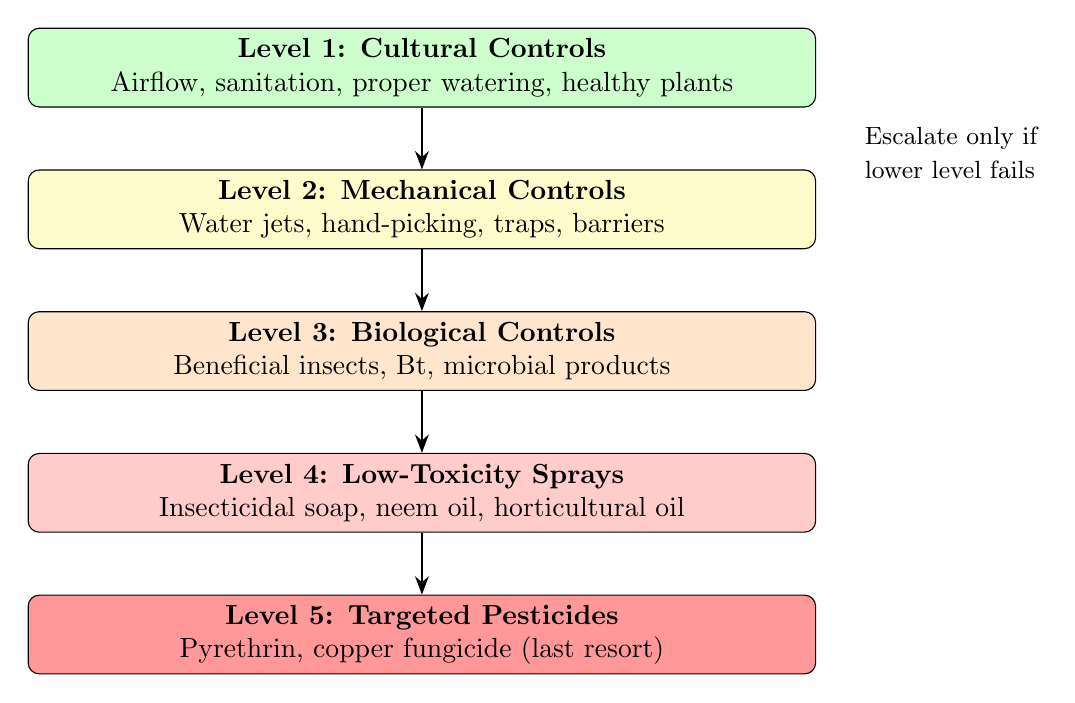
\begin{tikzpicture}[
  level/.style={rectangle, rounded corners, draw, minimum width=10cm, minimum height=1cm, align=center},
  arrow/.style={-{Stealth}, thick}
]
  \node[level, fill=green!20] (l1) at (0,0) {\textbf{Level 1: Cultural Controls}\\Airflow, sanitation, proper watering, healthy plants};
  
  \node[level, fill=yellow!20] (l2) at (0,-1.8) {\textbf{Level 2: Mechanical Controls}\\Water jets, hand-picking, traps, barriers};
  
  \node[level, fill=orange!20] (l3) at (0,-3.6) {\textbf{Level 3: Biological Controls}\\Beneficial insects, Bt, microbial products};
  
  \node[level, fill=red!20] (l4) at (0,-5.4) {\textbf{Level 4: Low-Toxicity Sprays}\\Insecticidal soap, neem oil, horticultural oil};
  
  \node[level, fill=red!40] (l5) at (0,-7.2) {\textbf{Level 5: Targeted Pesticides}\\Pyrethrin, copper fungicide (last resort)};
  
  \draw[arrow] (l1.south) -- (l2.north);
  \draw[arrow] (l2.south) -- (l3.north);
  \draw[arrow] (l3.south) -- (l4.north);
  \draw[arrow] (l4.south) -- (l5.north);
  
  \node[right] at (5.5,-0.9) {\small Escalate only if};
  \node[right] at (5.5,-1.3) {\small lower level fails};
\end{tikzpicture}
\end{center}

\subsection{Rodent Management (Ground-Level Specific)}

\begin{itemize}
  \item Install 1/4-inch hardware cloth barriers around container bases
  \item Use slings to keep fruit elevated off surfaces
  \item Remove fallen fruit and debris promptly
  \item Consider exclusion netting around ripening fruit
  \item Deploy snap traps in concealed locations if damage occurs
  \item Never use rodent poison near food crops
\end{itemize}

% =============================================================================
% SECTION 11: TROUBLESHOOTING
% =============================================================================
\section{Troubleshooting Guide}

\begin{longtable}{p{3.5cm}p{4.5cm}p{5.5cm}}
\toprule
\textbf{Problem} & \textbf{Likely Causes} & \textbf{Corrective Actions} \\
\midrule
\endhead

\multicolumn{3}{l}{\textbf{Germination and Seedling Issues}} \\
\midrule
Seeds fail to germinate & Soil too cold; old seeds; too wet & Verify 80--85\degree F soil temp; use fresh seed; reduce moisture \\
\addlinespace
Leggy seedlings & Insufficient light; too warm & Lower temps after emergence; increase light intensity; lower fixtures \\
\addlinespace
Damping off & Fungal disease; overwatering & Use sterile mix; improve drainage; reduce humidity; discard affected seedlings \\
\midrule

\multicolumn{3}{l}{\textbf{Vegetative Growth Issues}} \\
\midrule
Slow growth & Cold temps; nutrient deficiency; root problems & Verify soil temps 65\degree F+; check feeding schedule; inspect roots \\
\addlinespace
Yellow leaves (older) & Nitrogen deficiency; overwatering & Increase N fertilizer; check drainage; reduce watering \\
\addlinespace
Yellow leaves (newer) & Iron deficiency; high pH & Chelated iron application; test and lower pH if needed \\
\addlinespace
Purple leaves & Phosphorus deficiency; cold stress & Bone meal application; protect from cold nights \\
\addlinespace
Wilting (despite water) & Root rot; bacterial wilt; heat stress & Check roots; test for wilt; provide afternoon shade \\
\midrule

\multicolumn{3}{l}{\textbf{Flowering and Fruit Set Issues}} \\
\midrule
No female flowers & Plant too young; excess nitrogen & Wait 2--3 more weeks; reduce N feeding; ensure adequate sun \\
\addlinespace
Flowers but no fruit & Poor pollination; heat stress & Hand-pollinate daily; pollinate in early AM; provide shade \\
\addlinespace
Fruit drops when small & Incomplete pollination; stress; too many fruits & Improve pollination; stabilize water; thin to 2 per plant \\
\addlinespace
Blossom end rot & Calcium deficiency; inconsistent watering & Calcium application; maintain even moisture; mulch \\
\midrule

\multicolumn{3}{l}{\textbf{Fruit Quality Issues}} \\
\midrule
Small fruit & Too many fruits; insufficient nutrition; water stress & Thin to 1--2 per plant; increase feeding; maintain moisture \\
\addlinespace
Bland/low sugar & Too many fruits; overwatering; insufficient sun & Aggressive thinning; reduce water pre-harvest; maximize sun \\
\addlinespace
Fruit cracking & Inconsistent watering; rapid growth after drought & Maintain even moisture; gradual watering increases \\
\addlinespace
Misshapen fruit & Poor pollination; insect damage; physical obstruction & Improve pollination; pest control; adjust sling fit \\
\midrule

\multicolumn{3}{l}{\textbf{Environmental Issues}} \\
\midrule
Heat stress symptoms & Temps above 95\degree F; container overheating & Afternoon shade cloth; mulch; paint pots white; increase water \\
\addlinespace
Wind damage & Inadequate trellis support; exposed location & Reinforce trellis; add wind break; check tie security \\
\addlinespace
Container too dry & Undersized pot; poor water retention & Upsize container; add water-holding amendments; drip irrigation \\
\bottomrule
\end{longtable}

% =============================================================================
% SECTION 12: WEATHER CONTINGENCIES
% =============================================================================
\section{Weather Contingency Plans}

\subsection{Heat Wave Response (95\degree F+ for 3+ Days)}

\begin{procedurebox}[Heat Wave Protocol]
\begin{enumerate}
  \item Deploy shade cloth (30--50\% shade) during afternoon hours (12--5 PM)
  \item Increase watering frequency; may need twice-daily during extreme heat
  \item Apply additional mulch to reduce soil temperature
  \item Mist foliage in early morning only (not during hot afternoon)
  \item Suspend fertilizer applications until temperatures moderate
  \item Expect reduced fruit set; pollinate in early morning only (before 8 AM)
  \item Monitor for spider mites which thrive in hot, dry conditions
\end{enumerate}
\end{procedurebox}

\subsection{Drought Period Response}

\begin{itemize}
  \item Prioritize deep watering over frequent light watering
  \item Check moisture twice daily during extended dry periods
  \item Consider temporary drip system if not already installed
  \item Reduce fertilizer concentration to prevent salt buildup
  \item Accept slower growth; avoid panic overwatering
\end{itemize}

\subsection{Heavy Rain/Storm Response}

\begin{itemize}
  \item Ensure drainage holes are clear before storm arrives
  \item Tilt or elevate containers if flooding expected
  \item Stake and tie vines securely before high winds
  \item Cover containers with plastic to prevent waterlogging if extreme rain forecast
  \item Inspect trellis integrity immediately after storm
  \item Apply preventive fungicide if extended wet period follows
\end{itemize}

\subsection{Late Season Cold Snap}

\begin{itemize}
  \item Monitor forecasts closely from October onward
  \item Have frost cloth or row cover ready for deployment
  \item Harvest any mature fruit before cold event
  \item Cover plants completely; anchor covers to prevent wind lifting
  \item Water soil the day before frost (moist soil holds heat better)
  \item Consider string lights or other heat source under cover for borderline temps
\end{itemize}

% =============================================================================
% SECTION 13: POST-HARVEST
% =============================================================================
\section{Post-Harvest Handling and Storage}

\subsection{Immediate Post-Harvest Care}

\begin{enumerate}
  \item Allow freshly harvested fruit to rest in shade for 1--2 hours
  \item Do not wash exterior unless visibly dirty; moisture promotes decay
  \item If washing necessary, dry thoroughly and allow to air dry completely
  \item Handle with care; Bradford rinds bruise easily
  \item Store stem-side up to prevent moisture accumulation at stem attachment
\end{enumerate}

\subsection{Storage Recommendations}

\begin{table}[H]
\centering
\caption{Storage Guidelines}
\begin{tabular}{@{}p{4cm}p{3.5cm}p{6cm}@{}}
\toprule
\textbf{Storage Method} & \textbf{Duration} & \textbf{Notes} \\
\midrule
Room temperature & 7--14 days & Best flavor; out of direct sun \\
Cool room (55--60\degree F) & 2--3 weeks & Extends storage; slightly reduces flavor \\
Refrigerated (whole) & Not recommended & Causes flesh deterioration; chilling injury \\
Refrigerated (cut) & 3--5 days & Wrap tightly in plastic; consume promptly \\
\bottomrule
\end{tabular}
\end{table}

\subsection{Quality Assessment}

\begin{itemize}
  \item \textbf{Visual:} Deep red flesh color; no white streaking; minimal seed cavity
  \item \textbf{Texture:} Fine-grained; firm but not hard; no mealiness
  \item \textbf{Taste:} Intense sweetness; complex flavor; no off-tastes
  \item \textbf{Brix measurement:} Cut small sample from center; test with refractometer; target 11\degree+ for Bradford quality
\end{itemize}

\subsection{Seed Saving (Optional)}

Bradford watermelons are open-pollinated heirlooms, allowing seed saving for future seasons:

\begin{enumerate}
  \item Select seeds from your best-tasting, well-formed fruit
  \item Scoop seeds into bowl; remove as much flesh as possible
  \item Rinse thoroughly in strainer under running water
  \item Spread seeds in single layer on paper towel or screen
  \item Dry in warm, well-ventilated area for 1--2 weeks
  \item Seeds are fully dry when they snap rather than bend
  \item Store in paper envelope inside airtight container with desiccant
  \item Label with variety, date, and any notes
  \item Properly stored seeds remain viable for 4--5 years
\end{enumerate}

% =============================================================================
% SECTION 14: RECORDKEEPING
% =============================================================================
\section{Recordkeeping and Documentation}

\subsection{Essential Records to Maintain}

\begin{table}[H]
\centering
\caption{Growing Season Documentation Requirements}
\begin{tabular}{@{}p{4cm}p{9.5cm}@{}}
\toprule
\textbf{Record Type} & \textbf{Information to Capture} \\
\midrule
Seed Information & Source, lot number, purchase date, germination rate observed \\
Timeline & Seed start date, emergence date, transplant date, first flower, first fruit set, harvest dates \\
Fertilizer Log & Product used, rate, date applied, plant response notes \\
Irrigation Log & Frequency, duration, adjustments made, rainfall received \\
Pest/Disease Log & Date observed, pest/disease identified, severity, action taken, result \\
Pollination Log & Dates, flowers pollinated, success rate, fruit tagged \\
Environmental & Notable weather events, temperature extremes, protective actions \\
Harvest Record & Date, fruit weight, visual quality, taste assessment, Brix if measured \\
Post-Season Analysis & What worked, what failed, changes for next season \\
\bottomrule
\end{tabular}
\end{table}

\subsection{Sample Log Template}

\begin{verbatim}
DATE: ___________  WEEK: ___  DAYS SINCE TRANSPLANT: ___

WEATHER:
  High: ___°F  Low: ___°F  Conditions: _______________

IRRIGATION:
  Time: ________  Amount: ________  Notes: ___________

PLANT HEALTH (1-10): ___
  Observations: ____________________________________

PEST/DISEASE:
  Type: ____________  Location: ____________________
  Severity: Low / Medium / High
  Action: _________________________________________

FERTILIZER:
  Product: _____________  Rate: ____________________

OTHER NOTES:
  ________________________________________________
\end{verbatim}

% =============================================================================
% SECTION 15: PRE-FLIGHT READINESS
% =============================================================================
\section{Pre-Flight Readiness Review}

Complete this review during the week before transplanting. A ``No'' response on any \textbf{Go/No-Go} item should delay transplant until remediated.

\subsection{Go/No-Go Checklist}

\begin{longtable}{p{0.06\linewidth}p{0.54\linewidth}p{0.36\linewidth}}
\toprule
\textbf{} & \textbf{Readiness Item} & \textbf{Acceptance Criteria} \\
\midrule
\endhead

\multicolumn{3}{l}{\textbf{Environmental Readiness}} \\
\midrule
\cb & Sun exposure validated & 8+ hours direct sun confirmed in pot locations \\
\cb & Frost risk cleared & No frost in 10-day forecast; soil temp 65\degree F+ \\
\cb & Severe weather window & No major storms forecast for transplant week \\
\midrule

\multicolumn{3}{l}{\textbf{Container and Structure}} \\
\midrule
\cb & Containers sized and staged & 2 containers at 25--30 gal in final positions \\
\cb & Drainage verified & Water exits freely; pot feet installed \\
\cb & Trellis assembled and anchored & Rigid, 7+ ft; load tested; does not wobble \\
\cb & Sling materials ready & At least 4 slings prepared \\
\midrule

\multicolumn{3}{l}{\textbf{Growing Systems}} \\
\midrule
\cb & Irrigation plan tested & Soil-line delivery confirmed; timer tested if used \\
\cb & Growing media prepared & Quality mix + compost blended; pre-moistened \\
\cb & Fertilizer plan staged & Base fertilizer incorporated; liquid feeds on hand \\
\cb & Mulch materials ready & Straw or leaves staged for application \\
\midrule

\multicolumn{3}{l}{\textbf{Pest Management}} \\
\midrule
\cb & Monitoring deployed & Sticky cards placed; baseline recorded \\
\cb & IPM supplies stocked & Soap, neem, and spray equipment ready \\
\cb & Exclusion materials ready & Row cover/netting available if needed \\
\midrule

\multicolumn{3}{l}{\textbf{Plant Readiness}} \\
\midrule
\cb & Seedlings meet quality gate & 2--3 true leaves, stocky, healthy color \\
\cb & Hardening complete & 7--10 days outdoor exposure completed \\
\cb & No visible pest/disease & Seedlings inspected and cleared \\
\midrule

\multicolumn{3}{l}{\textbf{Documentation}} \\
\midrule
\cb & Growing log prepared & Recording system ready for daily entries \\
\cb & Reference materials accessible & This run book and resources available \\
\bottomrule
\end{longtable}

\subsection{Decision Matrix}

\begin{center}
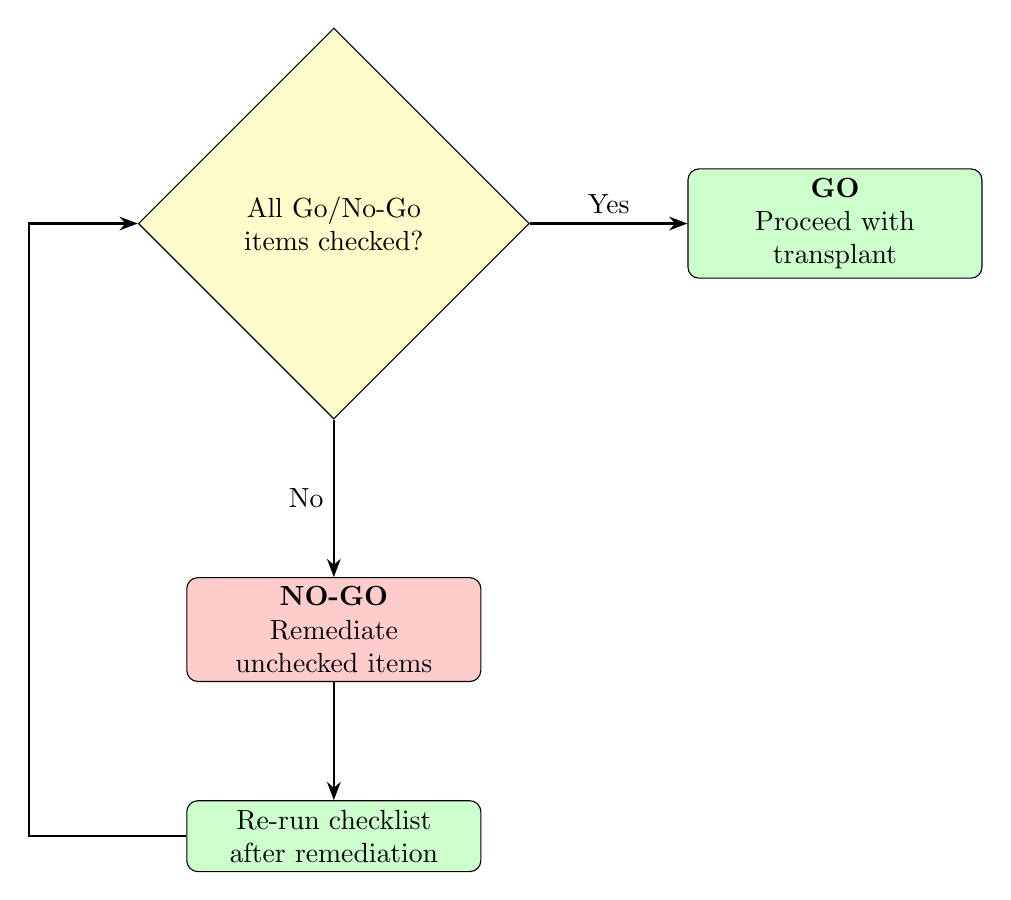
\begin{tikzpicture}[
  decision/.style={diamond, draw, fill=yellow!20, text width=4cm, align=center, inner sep=2pt},
  action/.style={rectangle, rounded corners, draw, fill=green!20, text width=3.5cm, align=center},
  stop/.style={rectangle, rounded corners, draw, fill=red!20, text width=3.5cm, align=center},
  arrow/.style={-{Stealth}, thick}
]
  \node[decision] (check) {All Go/No-Go items checked?};
  \node[action, right=2cm of check] (go) {\textbf{GO}\\Proceed with transplant};
  \node[stop, below=2cm of check] (nogo) {\textbf{NO-GO}\\Remediate unchecked items};
  \node[action, below=1.5cm of nogo] (recheck) {Re-run checklist\\after remediation};
  
  \draw[arrow] (check) -- node[above] {Yes} (go);
  \draw[arrow] (check) -- node[left] {No} (nogo);
  \draw[arrow] (nogo) -- (recheck);
  \draw[arrow] (recheck.west) -- ++(-2,0) |- (check.west);
\end{tikzpicture}
\end{center}

% =============================================================================
% SECTION 16: QUICK REFERENCE
% =============================================================================
\section{Quick Reference Summary}

\subsection{Key Numbers at a Glance}

\begin{table}[H]
\centering
\begin{tabular}{@{}p{6cm}p{7cm}@{}}
\toprule
\textbf{Parameter} & \textbf{Target Value} \\
\midrule
Container size & 25--30 gallons per plant \\
Plant count & 2 plants \\
Container spacing & 6--8 ft apart \\
Trellis height & 7--8 ft \\
Fruits per plant & 1--2 maximum \\
Seed starting date & March 10--20 \\
Transplant date & April 20--May 5 \\
Days to harvest & 85--100 from transplant \\
Harvest window & Mid-July through August \\
Germination temp & 80--85\degree F \\
Soil temp for transplant & 65\degree F minimum \\
Sun requirement & 8+ hours direct \\
Water frequency & Daily check; water when dry at 2--3 in \\
Fertilizer schedule & Weekly vegetative; every 10--14 days fruiting \\
\bottomrule
\end{tabular}
\end{table}

\subsection{Emergency Contacts and Resources}

\begin{itemize}
  \item \textbf{Local Extension Office:} Douglas County Extension (770-920-7224)
  \item \textbf{Weather Alerts:} weather.gov/atlanta
  \item \textbf{Bradford Seed Source:} bradfordwatermelons.com
  \item \textbf{Pest ID Help:} UGA Extension Pest Management Handbook (online)
\end{itemize}

% =============================================================================
% APPENDICES
% =============================================================================
\appendix
\section{Appendix A: Monthly Task Calendar}

\begin{table}[H]
\centering
\caption{Month-by-Month Activity Summary}
\begin{tabular}{@{}p{2cm}p{11.5cm}@{}}
\toprule
\textbf{Month} & \textbf{Primary Activities} \\
\midrule
March & Start seeds indoors (10--20); maintain seedlings; prepare containers and media; install trellis \\
April & Harden seedlings (1--20); transplant (20--30); establish plants; begin pest monitoring \\
May & Intensive vegetative care; vine training; weekly feeding; watch for pests \\
June & Flowering begins; hand-pollinate daily; fruit set decisions; install slings; transition fertilizer \\
July & Fruit development; weekly sling adjustment; reduce watering pre-harvest; watch for disease \\
August & Monitor ripeness; harvest as ready; continue care for remaining fruit; record keeping \\
September & Final harvests; seed saving if desired; season wrap-up; documentation review \\
\bottomrule
\end{tabular}
\end{table}

\section{Appendix B: Conversion Tables}

\begin{table}[H]
\centering
\caption{Useful Conversions}
\begin{tabular}{@{}ll@{}}
\toprule
\textbf{Measurement} & \textbf{Conversion} \\
\midrule
1 gallon container & Approximately 0.13 cubic feet of media \\
1 cubic foot & Approximately 7.5 gallons \\
30 gallon container & Approximately 4 cubic feet of media \\
1 tablespoon & 3 teaspoons \\
1 fluid ounce & 2 tablespoons \\
Temperature C to F & F = (C × 9/5) + 32 \\
Temperature F to C & C = (F - 32) × 5/9 \\
\bottomrule
\end{tabular}
\end{table}

\section{Appendix C: Fertilizer Mixing Guide}

\begin{table}[H]
\centering
\caption{Standard Dilution Rates}
\begin{tabular}{@{}p{4cm}p{3.5cm}p{6cm}@{}}
\toprule
\textbf{Concentration} & \textbf{Rate per Gallon} & \textbf{When to Use} \\
\midrule
1/4 strength & 1/4 tsp per gallon & Seedlings; stressed plants \\
1/2 strength & 1/2 tsp per gallon & Transplant week; recovery \\
Full strength & 1 tsp per gallon & Standard weekly feeding \\
\bottomrule
\end{tabular}
\end{table}

\textit{Note: Rates assume typical concentrated liquid fertilizer. Always verify with product label and adjust accordingly.}

\vspace{2cm}
\begin{center}
\rule{0.6\textwidth}{0.4pt}\\[0.5cm]
{\large\textit{End of Bradford Watermelon Balcony Run Book}}\\[0.3cm]
{\small Version 2.0 --- Enhanced Edition}\\[0.2cm]
{\small Document prepared for Lithia Springs, Georgia cultivation}
\end{center}

\end{document}
